% Тут используется класс, установленный на сервере Papeeria. На случай, если
% текст понадобится редактировать где-то в другом месте, рядом лежит файл matmex-diploma-custom.cls
% который в момент своего создания был идентичен классу, установленному на сервере.
% Для того, чтобы им воспользоваться, замените matmex-diploma на matmex-diploma-custom
% Если вы работаете исключительно в Papeeria то мы настоятельно рекомендуем пользоваться
% классом matmex-diploma, поскольку он будет автоматически обновляться по мере внесения корректив
%

% По умолчанию используется шрифт 14 размера. Если нужен 12-й шрифт, уберите опцию [14pt]
%\documentclass[14pt]{matmex-diploma}
\documentclass[14pt]{matmex-diploma-custom}
\usepackage{graphicx}
\usepackage{multirow}

\begin{document}
\def\figurename{Рис}

% Год, город, название университета и факультета предопределены,
% но можно и поменять.
% Если англоязычная титульная страница не нужна, то ее можно просто удалить.
\filltitle{ru}{
    chair              = {Математическое обеспечение и администрирование \\ информационных систем \\ \vspace{5mm} Системное программирование},
    title              = {Комбинирование нейронных сетей и синтаксического анализа для обработки вторичной структуры последовательностей},
    % Здесь указывается тип работы. Возможные значения:
    %   coursework - Курсовая работа
    %   diploma - Диплом специалиста
    %   master - Диплом магистра
    %   bachelor - Диплом бакалавра
    type               = {diploma},
    position           = {студента},
    group              = 444,
    author             = {Лунина Полина Сергеевна},
    supervisorPosition = {к.\,ф.-м.\,н., доцент},
    supervisor         = {Григорьев С.\,В.},
    reviewerPosition   = {Специалист по анализу данных ООО "Интеллоджик"},
    reviewer           = {Малыгина Т.\,С.},
    chairHeadPosition  = {д.\,ф.-м.\,н., профессор},
    chairHead          = {Терехов А.\,Н.},
%   university         = {Санкт-Петербургский Государственный Университет},
%   faculty            = {Математико-механический факультет},
%   city               = {Санкт-Петербург},
%   year               = {2018}
}
\filltitle{en}{
    type               = {diploma},
    chair              = {Software and Administration of Information Systems \\ \vspace{5mm} Software Engineering},
    title              = {The composition of neural networks and parsing for secondary structure processing},
    author             = {Polina Lunina},
    supervisorPosition = {Assistant Professor},
    supervisor         = {Semyon Grigorev},
    reviewerPosition   = {Data scientist at Intellogic LLC},
    reviewer           = {Tatiana Malygina},
    chairHeadPosition  = {Professor},
    chairHead          = {Andrey Terekhov},
}
\maketitle
\tableofcontents
% У введения нет номера главы
\section*{Введение}
В совершенно разных предметных областях встречаются концептуально схожие задачи, связанные с анализом различных символьных цепочек. Например, распознавание и классификация геномных последовательностей в биоинформатике или поиск аномалий в цепочках системных вызовов в компьютерной безопасности. Часто оказывается, что исследуемые последовательности обладают достаточно специфической синтаксической структурой и, учитывая некоторым способом ее особенности при разработке алгоритмов для решения различных задач, можно значительно повысить их точность и эффективность. Применительно к биологии, синтаксическими структурами можно, в частности, описать вторичную структуру макромолекул. Далее мы будем называть такие синтаксические структуры вторичными структурами в том смысле, что они являются следующим уровнем организации после символьных цепочек. И это определение может применяться не только в биологической области, но и в иных сферах применения.
 
Одним из классических способов описания вторичной структуры являются формальные грамматики. Они обладают широкими выразительными возможностями и позволяют описать связь между символами, находящимися на большом расстоянии. Например, как показали исследования в области биоинформатики, с помощью контекстно-свободных стохастических грамматик можно смоделировать синтаксическую структуру всей цепочки~\cite{dowell2004rna,PCFG}. Тем не менее, в общем случае создание такой грамматики --- достаточно сложная, а иногда и невозможная задача. Поэтому имеет смысл использовать более простую грамматику для описания только ключевых особенностей вторичной структуры, а для ее полноценного анализа применять другие методы.

Существенной проблемой при работе с реальными данными является возможное присутствие различного рода шумов, мутаций и случайных всплесков, что делает точные методы неприменимыми. Распространенный способ обработки таких данных --- использование методов машинного обучения, в особенности, искусственных нейронных сетей. Кроме того, нейронные сети предоставляют возможность эффективно находить сложные и не поддающиеся формализации структурные закономерности во входных данных.

В данной работе мы предлагаем новый подход для класса проблем, связанных с обработкой символьных данных, обладающих некоторой синтаксической структурой. Основная идея подхода --- комбинация методов синтаксического анализа и машинного обучения. Мы используем грамматику для описания основных особенностей синтаксической структуры, извлекаем эти особенности с помощью алгоритмов синтаксического анализа и обрабатываем полученные данные с помощью нейронных сетей, сконструированных и обученных для решения конкретной задачи. 

\section{Постановка задачи}
Целью данной работы является разработка подхода для анализа вторичной структуры последовательностей с использованием комбинации синтаксического анализа и нейронных сетей.

Для достижения данной цели в рамках работы были поставлены следующие задачи.
\begin{itemize}
    \item Разработать архитектуру решения, независимую от конкретной области применения и используемых технологий.
    \item Провести экспериментальные исследования.
\end{itemize}

\section{Обзор областей применения}
\subsection{Биоинформатика}
Одной из областей, где необходим анализ большого количества символьных последовательностей, является биоинформатика. Точные и эффективные методы для решения таких задач, как распознавание и классификация организмов по их генетическим данным, предсказание функций и вторичной структуры белков, аннотация геномов и т.п. стали ключевыми направлениями в современной вычислительной геномике (протеомике). 

Материалом для изучения являются нуклеотидные (или, в случае белков, аминокислотные) последовательности, некоторые участки которых соединяются между собой по определенным закономерностям, образуя сложную и стабильную вторичную структуру (рис.~\ref{molekula}).

\begin{figure}[h]
\begin{center}
\centering
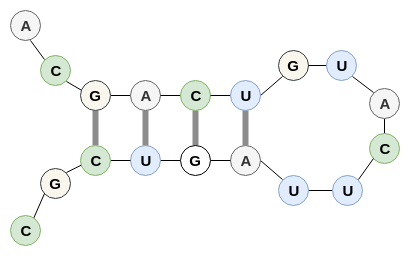
\includegraphics[width=8cm]{pics/molekula.png}
\caption{Образование вторичной структуры молекулы РНК}
\label{molekula}
\end{center}
\end{figure}    
Идея о том, что именно особенности вторичной структуры генетических цепочек существенны для решения задач распознавания и классификации, описана в различных научных работах и широко используется на практике~\cite{miladi2017rnascclust, vrehakova2014variation}.
Существующие подходы к описанию и моделированию вторичной структуры основаны на различных концепциях и алгоритмах, таких как скрытые марковские модели, ковариационные модели~\cite{EddyDurbin} и формальные грамматики~\cite{LWPCFG,PCFG,GrammarsRNA}. Распространенные проблемы при реализации данных подходов заключаются в больших временных затратах и теоретической сложности создания точной грамматики или модели. Тем не менее, многие их этих подходов успешно применяются на практике для разработки различных инструментов~\cite{hmmer,infernal}.

Концептуально другим подходом к решению задач биоинформатики является использование методов машинного обучения~\cite{ANN,Humidor}. Они позволяют находить сложные закономерности в больших объемах данных и учитывать характерную для биологических данных зашумленность.

Предложенный в данной работе подход позволяет, во-первых, совместить преимущества подходов, основанных на задании вторичной структуры и на машинном обучении, а во-вторых, повысить производительность этапа синтаксического анализа, так использование грамматики только для описания характерных особенностей вторичной структуры вместо классического способа (моделирования структуры всей цепочки) позволит существенно сократить размер грамматики и, как следствие, время, затраченное на работу парсера.

\subsection{Компьютерная безопасность}
Еще одной потенциальной областью применения предложенного подхода является компьютерная безопасность. Одна из самых острых проблем в данной области --- борьба с вредоносными программами. Для обнаружения их воздействия на систему применяют различные подходы, заключающиеся в поиске аномалий в последовательностях системных вызовов (трассах), совершенных другими программами ~\cite{ghosh1999study,hofmeyr1998intrusion,wespi2000intrusion}. Для этого нужно реализовать способ идентификации процессов, т.е. по некоторому набору особенностей научиться различать трассы различных программ и выявлять вирусы и отклонения. Трассы представляют из себя некоторые последовательности символов, в которых присутствуют закономерности, характерные для определенных видов программ, следовательно, формальное описание этих закономерностей может оказаться полезным при исследовании системных аномалий.

В работах~\cite{баклановский2015поведенческая,баклановский2016оценка} описан алгоритм обнаружения процессов вредоносных программ, основанный на поиске в трассах некоторых характерных шаблонов, по которым для набора процессов строятся описывающие их модели. Для каждого нового процесса проводится специальная оценка и подбирается наиболее близкая модель из существующих. Затем составляется вектор характеристик, оценивающих поведение процесса в рамках модели и подобные вектора используются для обучения нейронной сети, осуществляющей бинарную классификацию: процессы легитимных и вредоносных программ.

Описанная выше схема использует примерно те же идеи, что лежат в основе предложенного в данной работе подхода. В рамках нашего решения для создания модели понадобятся конъюнктивные грамматики, так как в трассах системных вызовов часто присутствуют повторяющиеся конструкции, выразимые в данном классе грамматик.

\section{Разработка архитектуры решения}
В данном разделе сначала представлена общая схема предложенного подхода, а затем детально описаны все части архитектуры решения. 
\subsection{Описание предложенного подхода}
Предложенный в данной работе подход может использоваться для решения различных задач во многих исследовательских областях. Ограничения, накладываемые на потенциальную область для апробации подхода, следующие. Во-первых, исследуемые данные --- некоторый набор символьных последовательностей с метаданными, для которых нужно решить задачу классификации по каким-либо признакам. Во-вторых, на основе анализа специфики области исследования и визуального изучения некоторого подмножества последовательностей можно выделить определенные характерные шаблоны и закономерности в их образовании, т.е. синтаксическую структуру. 

Процесс проведения эксперимента состоит из нескольких основных шагов. Сначала создается грамматика, описывающая характерные особенности вторичной структуры рассматриваемых последовательностей. Затем эти особенности извлекаются путем применения некоторого алгоритма синтаксического анализа ко входным данным по заданной грамматике. Результат его работы для входной строки и фиксированного нетерминала грамматики представим в виде булевой матрицы разбора, кодирующей информацию о выводимости подстрок данной строки из этого нетерминала. Такие матрицы приводятся к удобному для дальнейшей обработки виду и подаются на вход нейронной сети, осуществляющей классификацию в соответствии с условиями поставленной задачи. Кроме того, в процессе работы могут понадобиться некоторые дополнительные действия по обработке данных, уникальные для конкретного эксперимента, например, составление выборки, фильтрация и т.п.

Для удобства использования предложенного подхода на практике было необходимо унифицировать и задокументировать все шаги от начальной обработки данных до фиксации результатов. Необходимая для реализации подхода архитектура представлена на рис.~\ref{arch} и состоит из следующих частей.
\begin{itemize}
    \item Грамматика в принимаемом используемым инструментом для парсинга формате.
    \item База данных, хранящая сами входные последовательности, метаданные, результат парсинга, различные промежуточные данные и т.д.
    \item Parsing Tool --- утилита для обработки данных синтаксическим анализатором с возможностью сохранения результата в различные форматы.
    \item Neural Networks --- модуль для обучения и тестирования нейронных сетей.
    \item Data Processing --- модуль для промежуточной обработки данных.
\end{itemize}

\begin{figure}[h]
\begin{center}
\centering
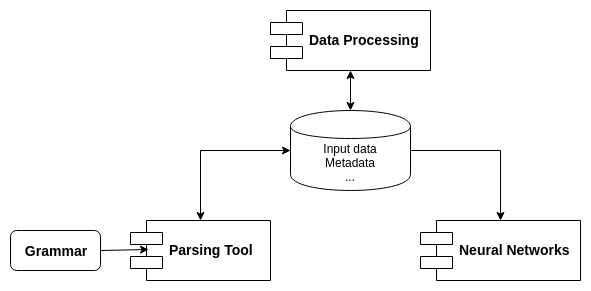
\includegraphics[width=14cm]{pics/arch.png}
\caption{Архитектура решения}
\label{arch}
\end{center}
\end{figure}    

В следующих разделах будут детально описаны все шаги по использованию предложенного подхода.

\subsection{Подготовка входных данных}

В данном разделе описаны необходимые для использования 
предложенного подхода данные, а также детали их хранения и представления. В процессе апробации подхода были выведены некоторые общие требования, позволяющие наиболее эффективно и удобно проводить экспериментальные исследования. 

Все необходимые данные помещаются в некоторое облачное хранилище, откуда могут извлекаться по мере необходимости. Входные данные --- исследуемые цепочки --- последовательно записаны в файлы формата fasta (для, например, биологических данных) или любого аналогичного текстового формата, причем каждой цепочке соответствует уникальный числовой идентификатор. Вся остальная информация о цепочках (метаданные, принадлежность к тестовой или обучающей выборке, класс и др.) хранится в специальной ссылочной таблице с доступом по идентификатору. 

Кроме того, в процессе исследования могут понадобиться специфические скрипты для промежуточной обработки данных, например, выборка для обучения нейронной сети, выравнивание цепочек до фиксированной длины, фильтрация входных данных и др. Эти скрипты реализуются в модуле Data Processing и могут быть переиспользованы в похожих экспериментах.

\subsection{Генерация данных с помощью синтаксического анализатора}
В рамках предложенной архитектуры синтаксический анализатор --- консольная утилита, принимающая на вход грамматику, файл с цепочками и список желаемых выходных форматов. Опишем основные принципы его работы.

Синтаксический анализ --- процесс проверки выводимости некоторой подстроки в заданной грамматике. В контексте предложенного решения терминальными символами грамматики являются символы исследуемых последовательностей, правила грамматики описывают характерные особенности их вторичной структуры, а алгоритм синтаксического анализа используется для извлечения этих особенностей путем поиска всех выводимых подстрок для данной строки для всех нетерминалов. Наш подход не зависит от выбора конкретного алгоритма синтаксического анализа, однако в описанных ниже экспериментах мы предлагаем использовать разработанный в рамках проекта YaccConstructor~\cite{yacc} в лаборатории JetBrains~\cite{jetbrains} алгоритм, основанный на матричных операциях~\cite{Azimov:2018:CPQ:3210259.3210264}, который демонстрирует высокую производительность на практике в связи с использованием параллельных вычислений.

Результат работы матричного синтаксического анализатора для входной строки $w$ и фиксированного нетерминала  $N$ --- верхнетреугольная булева матрица разбора $M_N$, хранящая информацию о всех подстроках, выводимых из $N$. Таким образом, $M_N[i,j]=1$, если подстрока $w[i,j-1]$  выводима из $N$. В зависимости от задачи и принципов построения грамматики для дальнейшей обработки могут быть выбраны различные нетерминалы. Мы предлагаем использовать такие матрицы как входные данные нейронной сети, поэтому необходимо привести их к удобному для обработки формату, учитывая специфику конкретной задачи. На данный момент в рамках расширения используемого алгоритма реализованы два формата преобразования матриц.
\begin{itemize}
    \item Вектора характеристик, сохраняемые в виде строк csv-файла. Генерация векторов осуществляется следующим образом: отбрасывается пустая часть матрицы ниже главной диагонали, оставшиеся строки последовательно преобразуются в битовый вектор, а затем сжимаются в байтовый вектор.
    \item Черно-белые изображения в формате bmp, получаемые путем замены нулевых битов матрицы на белые пиксели, а единичных --- на черные.
\end{itemize}
Кроме того, в исходный код инструмента можно легко добавить другие выходные форматы.

Классификация как векторов характеристик, так и изображений относится к классическим сценариям использования нейронных сетей, однако стоит отметить, что ввиду специфики конкретной задачи и особенностей входных цепочек, выбор формата данных может повлиять на эффективность и скорость обучения. Например, в процессе экспериментальных исследований было обнаружено, что, несмотря на то, что векторные данные занимают меньше памяти, их использование предполагает выравнивание всех цепочек до одинаковой длины, что может оказаться не самым эффективным решением для задач, где входные последовательности имеют принципиально разные длины, так как большая часть вектора для коротких цепочек в данном случае будет заполнена незначащими нулями. Изображения же можно сгенерировать для цепочек разных длин и затем привести к одному размеру, что позволяет аккуратно сохранить особенности вторичной структуры даже для коротких цепочек, однако это вызывает необходимость хранения больших объемов данных.

\subsection{Обучение нейронных сетей}
Искусственные нейронные сети --- широко применяемый метод решения задач классификации в областях, где входные данные обладают сложно формализуемыми закономерностями и могут содержать шумы и неточности. Мы предлагаем использовать нейронные сети для обработки сгенерированных синтаксическим анализатором данных, предполагая, что в них закодированы существенные для классификации особенности синтаксической структуры.

Архитектура нейронной сети уникальна для каждой конкретной задачи и предметной области, однако экспериментальные исследования выявили некоторые общие закономерности и интуиции. Для векторизованных данных высокую эффективность показало чередование полносвязных (dense) слоев ввиду утери информации о взаимном расположении элементов изначальной битовой матрицы и дропаут (dropout) слоев с нормализацией для стабилизации процесса обучения. Кроме того, при генерации векторов производится сжатие битовой матрицы в числовой вектор, что требует большего количества эпох при обучении, так как нейронной сети необходимы дополнительные действия для разжатия данных. Для изображений мы предлагаем использовать небольшое количество сверточных слоев (так как они применяются в основном для извлечения каких-либо особенностей из входных данных, а в нашем случае это уже сделано на этапе синтаксического анализа), затем линеаризацию, а далее перейти к чередующимся dense и dropout слоям, аналогично архитектуре для веторизованных данных. В качестве алгоритма оптимизации мы предлагаем использовать adagrad (adaptive gradient), позволяющий выделить редко встречающиеся особенности входных данных, которые, тем не менее, могут оказаться достаточно информативными для решения поставленных задач.

Выше был описан стандартный в рамках нашего подхода способ использования нейронных сетей, однако возможны различные его модификации, основанные на конструировании более сложных моделей с загрузкой весов уже обученных, что позволяет упростить задачу или повысить точность результата. Например, расширение нижней части нейронной сети слоями с большим количеством нейронов позволяет провести классификацию на большее количество классов, а расширение верхней части предоставляет возможность подачи на вход данных в другом формате, например, изначальной символьной последовательности вместо результата работы парсера.

Остановимся подробнее на последней модификации. Большинство алгоритмов синтаксического анализа работают за полином от длины входа, поэтому генерация большого количества данных на длинных цепочках потребует существенных временных затрат. Поэтому мы предлагаем следующую идею.
\begin{itemize}
    \item Сгенерировать некоторый набор данных с помощью синтаксического анализатора и обучить на них нейронную сеть (NN1).
    \item Создать новую нейронную сеть (NN2), которая расширяет вход NN1 несколькими слоями, верхний из которых принимает\linebreak символьные цепочки.
    \item Подгрузить веса NN1 на нижнюю часть NN2 и дообучить NN2.
\end{itemize}

Эта идея может быть применена как к векторизованным данным, так и к изображениям. В случае изображений необходимо использовать веса NN1, начиная с линеаризованного слоя. Таким образом можно, во-первых, уменьшить размер выборки для генерации парсером, а во-вторых, улучшить точность уже обученных нейронных сетей без временных затрат на дополнительную генерацию данных. Высокая точность и скорость обучения такой нейронной сети была подтверждена экспериментальным путем. 

\section{Эксперименты}
В данном разделе приведены результаты апробации предложенного подхода применительно к некоторым задачам биоинформатики, связанным с классификацией транспортных РНК (тРНК), цепочки которых представляют из себя последовательности символов алфавита\linebreak \{A, C, G, T\}, а синтаксической структурой являются закономерности образования вторичной (в биологическом смысле) структуры молекулы РНК. 

Контекстно-свободная грамматика в формате yard, использованная во всех приведенных далее экспериментах, приведена на рис.~\ref{rna}. Грамматика описывает основные структурные элементы вторичной структуры РНК --- стемы и петли.

\vspace{10}
\begin{figure} [h]
\begin{verbatim}
s1: stem<s0>
any_str : any_smb*[2..10]
s0: any_str | any_str stem<s0> s0
any_smb: A | T | C | G
stem1<s>: A s T | G s C | T s A | C s G 
stem2<s>: stem1< stem1<s> >
stem<s>:  
      A stem<s> T 
    | T stem<s> A 
    | C stem<s> G 
    | G stem<s> C 
    | stem1< stem2<s> >  
\end{verbatim}
\caption{Контекстно-свободная грамматика, описывающая особенности вторичной струкутры РНК}
\label{rna}
\end{figure}

В описанных далее экспериментах поставлены следующие задачи: классификация тРНК на 2 класса (эукариоты и прокариоты) и на 4 класса (археи, бактерии, растения и грибы).

Как было упомянуто в разделе 3.3, в существующем инструменте для синтаксического анализа существует два формата выходных данных: изображения и числовые вектора. Кроме того, в разделе 3.4 была описана идея расширения обученных нейронных сетей верхними слоями, принимающими на вход исходную символьную последовательность, а не результат работы парсера. На основе этих соображений, для поставленных выше задач были проведены два типа экспериментов на одних и тех же данных: обучение нейронной сети на векторизованных данных с последующим дообучением до строкового входа и аналогично для изображений.


Для создания и обучения нейронных сетей в данной работе были использованы библиотека Keras~\cite{keras} и фреймворк TensorFlow~\cite{tensorflow}.
Для оценки качества работы описанных далее нейронных сетей были использованы классические метрики, используемые в задачах машинного обучения. Введем некоторые обозначения.
\begin{itemize}
    \item $P$ --- общее количество образцов, по которым классификатор принял правильное решение, $N$ --- общее количество образцов, для которых класс был определен неверно.
    \item $TP_{c}$ (True Positive) --- количество образцов в пределах класса $c$, которые классификатор распознал как $c$.
    \item $FP_{c}$ (False Positive) --- количество образцов из выборки, которые были классифицированы как $c$, но при этом относятся к другому классу.
    \item $FN_{c}$ (False Negative) --- количество образцов из класса $c$, ошибочно отнесенных к другому классу.
\end{itemize}

На основе данных обозначений определим три метрики.
\begin{itemize}
    \item $Accuracy$ = $\frac{P}{N}$ ("правильность" --- доля правильно определенных классификатором образцов по всей тестовой выборке).
    \item $Precision_{c}$ = $\frac{TP_{c}}{TP_{c} + FP_{c}}$ ("точность" в пределах класса $c$ --- доля образцов, действительно принадлежащих $c$, относительно всех образцов, которые классификатор отнес к $c$).
    \item $Recall_{c}$ = $\frac{TP_{c}}{TP_{c} + FN_{c}}$  ("полнота" в пределах класса $c$ --- доля найденных классификатором образцов, принадлежащих $c$, относительно всех образцов этого класса в тестовой выборке).
\end{itemize}


\subsection{Классификация тРНК: эукариоты и прокариоты}
В данном эксперименте была поставлена задача бинарной классификации цепочек тРНК эукариотов и прокариотов (две группы, на которые разделяются все живые организмы в зависимости от наличия ядер в их клетках). Для обучения нейронных сетей было взято 35000 последовательностей из баз~\cite{trnadb1,trnadb2} в соотношении 20000:5000:10000  образцов на обучение, валидацию и тестирование соответственно, причем в каждой выборке было одинаковое количество образцов обоих классов.

\vspace{10}
\underline{Подход на основе векторизованных данных}

Перед генерацией векторов было необходимо выравнить цепочки до одной длины; мы выбрали верхнюю границу в 220 символов, так как, за исключением единичных случайных всплесков, большая часть последовательностей тРНК имеет меньшую длину. Для выравнивания цепочек был использован следующий алгоритм: если длина строки больше 220, то взять ее первые 220 символов, иначе добавить в конец необходимое количество специальных символов, не встречающихся в оригинальных цепочках, и учесть этот факт при создании грамматики.

На сгенерированных синтаксическим анализатором данных была обучена нейронная сеть (бинарный классификатор), состоящая из чередующихся dense и dropout слоев с нормализацией. Далее была сконструирована нейронная сеть, состоящая из двух блоков: входной слой с 220 нейронами и затем несколько полносвязных слоев, постепенно расширяющихся до длины вектора (3028), а затем --- слои вышеописанной нейронной сети, для которых при обучении были загружены уже посчитанные веса. Таким образом, на основе векторного классификатора был создан классификатор последовательностей тРНК, архитектура которого показана на рис.~\ref{nn1}, здесь правая часть --- модель нейронной сети, принимающей на вход векторизованные данные, а левая часть --- надстройка, преобразующая нуклеотидную последовательность в вектор.

\begin{figure} [h]
\begin{center}
\centering
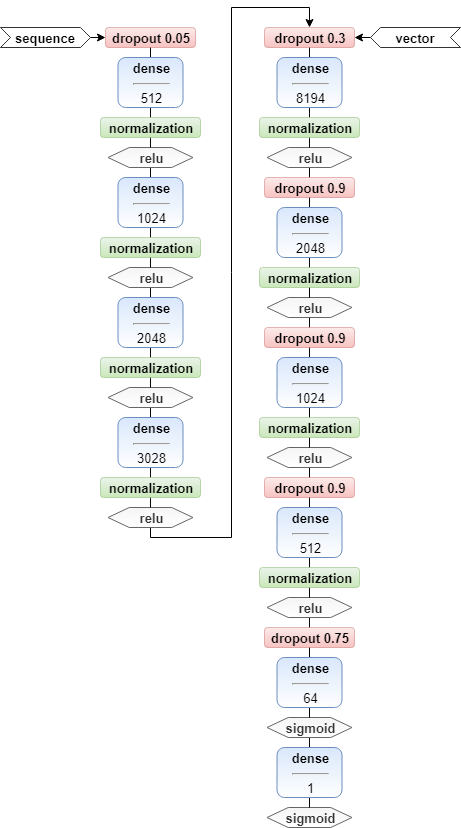
\includegraphics[width=8cm]{pics/nn.png}
\caption{Архитектура нейронной сети для классификации тРНК}
\label{nn1}
\end{center}
\end{figure}  

\vspace{10}
\underline{Подход на основе изображений}

Результатом работы синтаксического анализатора на цепочке длины $N$ является изображение размера $N\times N$, поэтому унификацию размеров сгенерированных данных можно провести путем последующего приведения изображений к единому размеру, что позволяет обрабатывать последовательности разных длин без выравнивания.

В данном эксперименте на наборе сгенерированных и приведенных к размеру $80\times80$ данных была обучена нейронная сеть со входным сверточным слоем (convolution layer), линеаризацией (flatten), а затем, аналогично архитектуре для векторных данных, чередованием dense и dropout слоев. Далее, по той же схеме, что описано ранее, было реализовано расширение полученного классификатора до строкового входа. Единственное различие заключается в том, что из модели комбинированной нейронной сети был удален сверточный слой, таким образом, на стыке надстройки и обученной модели в данном случае находится слой линеаризации.

\vspace{10}
\underline{Результаты}

Результаты тестирования на тестовой выборке в 10000 образцов были оценены в соответствии с приведенными в начале раздела 4 метриками. В таблице~\ref{results_ep} показана оценка классификаторов по метрике $Accuracy$ до и после дообучения до строкового входа, а также суммарное время, затраченное на обучение. В таблице~\ref{metrics_ep} продемонстрированы результаты вычисления метрик $Precision$ и $Recall$ для обоих классов на расширенных моделях.
\vspace{10}
\begin{table}[h]
\begin{tabular}{|l|l|l|}
\hline
                        & vector-based approach & image-based approach \\ \hline
base model accuracy     & 94.1\%                & 96.2\%               \\ \hline
extended model accuracy & 97.5\%                & 97.8\%               \\ \hline
total training time     & 28300 s               & 6100 s               \\ \hline
\end{tabular}
\caption{Доля правильных ответов классификаторов и время обучения}
\label{results_ep}
\end{table}

\begin{table}[h]
\begin{tabular}{|l|l|l|l|l|}
\hline
\multirow{2}{*}{class} & \multicolumn{2}{l|}{vector-based approach} & \multicolumn{2}{l|}{image-based approach} \\ \cline{2-5} 
                       & precision             & recall             & precision             & recall            \\ \hline
prokaryotic            & 95.8\%                & 99.4\%             & 96.2\%                & 99.4\%            \\ \hline
eukaryotic             & 99.4\%                & 95.6\%             & 99.4\%                & 99.5\%            \\ \hline
average             & 97.6\%                & 97.5\%             & 97.8\%                & 99.5\%            \\ \hline
\end{tabular}
\caption{Сравнение результатов тестирования подходов по метриками precision и recall для каждого класса}
\label{metrics_ep}
\end{table}

\subsection{Классификация тРНК: археи, бактерии, растения и грибы}
В данном эксперименте была исследована возможность классификации цепочек тРНК на большее количество классов, менее крупных с точки зрения биологической систематики. Анализируемые последовательности в количестве 12000 образцов были взяты из тех же самых  баз~\cite{trnadb1,trnadb2} и поделены для обучения, валидации и тестирования в соотношении 8000:3000:1000 образцов соответственно, причем в каждой выборке было равное количество образцов каждого класса.

Аналогично эксперименту, описанному в предыдущем разделе, были обучены векторный классификатор и классификатор изображений с единственным различием в размере выходного слоя. Затем для обоих классификаторов было реализована надстройка, принимающая исходные цепочки. Время работы, а также различные оценки результатов, полученных при тестировании обоих мультиклассовых классификаторов по метрикам $Accuracy$, $Precision$ и $Recall$ приведены в таблицах~\ref{results_abfp} и~\ref{metrics_abfp}.
\begin{table}[h]
\begin{tabular}{|l|l|l|}
\hline
                        & vector-based approach & image-based approach \\ \hline
base model accuracy     & 86.7\%                & 93.3\%               \\ \hline
extended model accuracy & 96.2\%                 & 95.7\%               \\ \hline
total training time     & 36000 s               & 4200 s               \\ \hline
\end{tabular}
\caption{Доля правильных ответов классификаторов и время обучения}
\label{results_abfp}
\end{table}

\begin{table}[h]
\begin{tabular}{|l|l|l|l|l|}
\hline
\multirow{2}{*}{class} & \multicolumn{2}{l|}{vector-based approach} & \multicolumn{2}{l|}{image-based approach} \\ \cline{2-5} 
                       & precision             & recall             & precision             & recall            \\ \hline
archaeal               & 91.1\%                & 99.2\%             & 91.6\%                & 98.5\%            \\ \hline
bacterial              & 96.6\%                & 95.1\%             & 95.2\%                & 95.5\%            \\ \hline
fungi                  & 98.5\%                & 94.9\%             & 97.5\%                & 94.3\%            \\ \hline
plant                  & 99.4\%                & 95.7\%             & 99.2\%                & 94.7\%            \\ \hline
average                  & 96.4\%                & 96.2\%             & 95.9\%                & 95.8\%            \\ \hline
\end{tabular}
\caption{Сравнение результатов тестирования подходов по метрикам precision и recall для каждого класса}
\label{metrics_abfp}
\end{table}

\subsection{Анализ результатов}
В результате экспериментов на генетических данных была доказана возможность применения комбинации синтаксического анализа и нейронных сетей к различным задачам биоинформатики.

Были исследованы два формата представления данных, хранящих информацию о вторичной структуре, и влияние выбора формата на процесс обучения нейронных сетей. На основе полученных результатов видно, что скорость обучения на изображениях в разы выше, чем на векторных данных при несущественных различиях в точности, так как в векторных данных нарушено взаимное расположение закодированных элементов вторичной структуры, а также сжатие информации при генерации вектора требует дополнительных действий по ее обработке при обучении. Тем не менее, в случае достаточно большой длины входной цепочки обучение нейронной сети на изображениях может привести к существенным затратам по времени и памяти вплоть до превышения ограничений на использование памяти GPU и CPU в фреймворках для машинного обучения. Кроме того, изображения требуют привлечения больших ресурсов для хранения.

Решение задач биоинформатики является частным и не единственным примером области исследования применимости предложенного подхода. В других областях могут потребоваться иные форматы представления данных и архитектуры нейронных сетей, более сложные грамматики и т.д.


\section*{Заключение}
В ходе данной работы были получены следующие результаты.
\begin{itemize}
    \item Разработана архитектура решения для использования предложенного подхода.
    \item Проведены экспериментальные исследования предложенного подхода на задачах классификации тРНК. 
    \item Опубликована статья "The Composition of Dense Neural Networks and Formal Grammars for Secondary Structure Analysis" на конференции BIOINFORMATICS 2019 и представлен постер "16s rRNA Detection by Using Neural Networks" на конференции Biata 2018.
    \item Исходный код и докуметация доступны по ссылке\linebreak https://github.com/LuninaPolina/SecondaryStructureAnalyzer.
\end{itemize}


Можно найти различные области и задачи для апробации предложенного подхода. Мы предлагаем два основных направления будущего развития. Во-первых, дальнейшие эксперименты в области биоинформатики.
\begin{itemize}
    \item Исследования аминокислотных последовательностей белков и особенностей образования их вторичной структуры для решения различных задач, в частности, предсказание функции белка (т.е. определение его биологической роли в организме, например, структурная, каталитическая, защитная и др.).
    \item Фильтрация биологических баз данных на предмет наличия в них химер, т.е. организмов, состоящих из генетически разнородных клеток.
    \item Моделирование вторичных структур геномных последовательностей.
\end{itemize}
 Во-вторых, различные эксперименты в области кибербезопасности, в частности, поиск аномалий в последовательностях системных вызовов.


% У заключения нет номера главы
%\section*{Coclusion}

\setmonofont[Mapping=tex-text]{CMU Typewriter Text}
\bibliographystyle{ugost2008ls}
\renewcommand\refname{Список литературы}
\bibliography{diploma.bib}
\end{document}
